\section*{Introduction}

\addcontentsline{toc}{section}{Introduction}
Le projet GE-S7 mêle les domaines de l'automatique et de l’électrotechnique dans le contexte de l'asservissement de machines à courant continu. En particulier, nous réaliserons un asservissement de courant et de vitesse en accord avec un cahier des charges établi au préalable. Ce projet va se dérouler en plusieurs étapes majeures que nous pouvons résumer de la manière suivante :

\begin{itemize}
    \item Étude du système à asservir
    \item Modélisation et simulation du système en boucle ouverte
    \item Dimensionnement et simulation des asservissements
    \item Conception et réalisation du circuit imprimé
    \item Tests réels et comparaison avec les simulations
\end{itemize}

Le projet a pour objectifs de réaliser l'asservissement d'une machine et d'en comprendre les enjeux à travers les différentes étapes décrites ci-dessus. Il nous permet de nous mettre dans un cadre concret pour développer des compétences qui seront importantes dans notre futur métier d'ingénieur et en particulier, la démarche de projet et le travail en équipe.

\vspace{0.5cm}

\textit{Nous serons amenés dans ce rapport à fournir de nombreuses captures d'écran. Pour éviter d’alourdir le document et  faciliter la lecture, nous indiquerons l'origine de chaque capture d'écran dans la \autoref{sec:arb} où le fichier d'origine de chaque figure sera indiquée. Il sera possible de s'y rendre en cliquant sur l’astérisque "*" présente à la fin de chaque titre de figure, et de revenir à la figure en cliquant sur le numéro de cette dernière dans l'arborescence.}

\vspace{2cm}

\section{Présentation des machines à courant continu utilisées}
\subsection{Fonctionnement général d'une machine à courant continu}
Une machine à courant continu est composée comme toute machine électrique tournante d'une partie fixe: le stator, et d'une partie rotative: le rotor. Le stator \textit{(ou inducteur)} consiste soit en un aimant permanent, soit en un électroaimant. Le rotor \textit{(ou induit)}, lui, est bobiné et va être traversé par un courant continu. \\
L'interaction entre le courant au rotor et le champ magnétique du stator va générer une force sur les conducteurs rotoriques  permettant la rotation de la machine. De plus, pour permettre à la machine de tourner et de ne pas se bloquer du fait de la polarité du champ magnétique, une pièce appelée "collecteur" permet d'inverser la polarité du courant traversant les enroulements lors de la rotation, permettant ainsi un mouvement continu de la machine. \\ \\
De ce fait, si nous alimentons l'induit de notre MCC avec un courant continu (et éventuellement l'inducteur si elle n'est pas à aimant permanent), nous fonctionnerons en mode \UB{moteur}, et à l'inverse, en appliquant un mouvement de rotation sur l'arbre de notre MCC, nous fonctionnerons en \UB{génératrice}. \\ \\
\textit{Dans ce rapport, nous abrégerons souvent "machine à courant continu" par MCC.}

\newpage

\subsection{Caractéristiques des machines}
Nous utiliserons donc dans ce projet deux machines \UB{identiques}. Une fonctionnera en moteur, l'autre en génératrice. Le type de machine utilisé est à \UB{aimant permanent}, il ne sera donc pas nécessaire d'alimenter l'inducteur. Les machines sont à deux paires de pôles et leurs caractéristiques sont listées dans le \autoref{tab:caract_mcc}.
\begin{table}[H]
    \centering
    \caption{Caractéristiques des MCC}
    \begin{tabular}{||c|c|c|c||}
        \hline
        Caractéristique                              & Valeur   & Unité                        & Symbole
        \\  \hline \hline
        Couple en rotation lente                     & 0,54     & $N.m$                        & $M_O$           \\
        \hline
        Courant nominal                              & 4,5      & $A$                          & $I$             \\
        \hline
        Tension nominale d'alimentation              & 49       & $V$                          & $U$             \\
        \hline
        Vitesse nominale                             & 3000     & $tr/min$                     & $N$             \\  \hline \hline
        Tension maximal                              & 65       & $V$                          & $U_{max}$       \\
        \hline
        Vitesse maximale                             & 4800     & $tr/min$                     & $N_{max}$       \\
        \hline
        Courant impulsionnel                         & 13       & $A$                          & $I_{max}$       \\
        \hline
        Fem par $1000~{tr/min}$ à 25\textdegree      & 13,3     & $\frac{V}{10^3\cdot tr/min}$ & $K_{e(tr/min)}$ \\
        \hline
        Coefficient de couple électromagnétique      & 0,127    & $N.m/A$                      & $K_\phi$        \\
        \hline
        Couple de frottement sec                     & 2,4      & $N.cm$                       & $T_f$           \\
        \hline
        Coefficient de viscosité par $1000~{tr/min}$ & 0,53     & $N.cm$                       & $K_d$           \\
        \hline
        Résistance de bobinage à 25\textdegree       & 1,52     & $\Omega$                     & $R$             \\
        \hline
        Inductance de bobinage                       & 2,2      & $mH$                         & $L$             \\
        \hline
        Inertie du rotor                             & 0,000083 & $kg.m^2$                     & $J$             \\
        \hline
        Constante de temps thermique                 & 7        & $min$                        & $T_{th}$        \\
        \hline
        Masse                                        & 1,34     & $kg$                         & $M$
        \\\hline
    \end{tabular}
    \label{tab:caract_mcc}
\end{table}

\subsection{Équations de fonctionnement}
Pour les besoins du projet, nous aurons besoin des équations de fonctionnement de la MCC en mode moteur. \\
À partir du schéma équivalent d'un moteur à courant continu illustré à la \autoref{circuit:sch_eq_MCC_moteur} et des équations de la mécanique, nous obtenons les équations de fonctionnement.

\begin{figure}[H]
    \centering
    \usetikzlibrary{shapes.geometric}
\begin{tikzpicture}
	% Paths, nodes and wires:
	\draw (1, -0.25) to[european resistor, l_={$R$}] (1, 1.75);
	\draw (1, 1.75) to[american inductor, mirror, l_={$L$}] (1, 3.75);
	\draw (1, -0.25) to[battery1, l={$E$}] (1, -1.75);
	\draw (1, 3.75) -- (-1.25, 3.75);
	\draw[-latex] (-2, 3.75) -- (-1.25, 3.75);
	\draw (1, -1.75) -- (-2, -1.75);
	\draw[-latex] (-2, -1.5) -- (-2, 3.5);
	\draw[-latex] (0.5, 2.25) -- (0.5, 3.25);
	\draw[-latex] (0.5, 0.25) -- (0.5, 1.25);
	\draw[-latex] (0.25, -1.5) -- (0.25, -0.5);
	\node[shape=rectangle, minimum width=0.715cm, minimum height=0.715cm] at (-2.25, 0.875){} node[anchor=north west, align=left, text width=0.327cm, inner sep=6pt] at (-2.625, 1.25){$U$};
	\node[shape=rectangle, minimum width=0.715cm, minimum height=0.715cm] at (0.125, 2.75){} node[anchor=north west, align=left, text width=0.327cm, inner sep=6pt] at (-0.25, 3.125){$U_L$};
	\node[shape=rectangle, minimum width=0.715cm, minimum height=0.715cm] at (0.125, 0.625){} node[anchor=north west, align=left, text width=0.327cm, inner sep=6pt] at (-0.25, 1){$U_R$};
	\node[shape=rectangle, minimum width=0.715cm, minimum height=0.715cm] at (-0.125, -1.125){} node[anchor=north west, align=left, text width=0.327cm, inner sep=6pt] at (-0.5, -0.75){$U_E$};
	\node[shape=rectangle, minimum width=0.715cm, minimum height=0.59cm] at (-1.625, 3.938){} node[anchor=north west, align=left, text width=0.327cm, inner sep=6pt] at (-2, 4.25){$I$};
	\node[shape=ellipse, draw={rgb,255:red,181;green,0;blue,}, line width=1pt, minimum width=3.965cm, minimum height=5.158cm] at (0.586, 0.903){};
	\node[shape=rectangle, minimum width=0.715cm, minimum height=0.715cm] at (1.375, 1.75){} node[anchor=north west, align=left, text width=0.327cm, inner sep=6pt] at (1, 2.125){\textcolor{rgb,255:red,181;green,0;blue,0}{Induit}};
\end{tikzpicture}
    \caption{Schéma équivalent d'un moteur à courant continu}
    \label{circuit:sch_eq_MCC_moteur}
\end{figure}

\begin{tcolorbox}[colback=yellow!5!white,colframe=yellow!50!black,
        colbacktitle=yellow!75!black,title= Équations de fonctionnement:]





    \begin{equation}
        \begin{array}{l}
            \text{\textbullet}~~ u(t)= e(t)+Ri(t)+L \frac{di(t)}{dt}  \\
            \text{\textbullet} ~~ J\frac{d\omega}{dt}=C_m(t)-C_{r}(t) \\
            \text{\textbullet} ~~ e(t)= K_e\omega(t)                  \\
            \text{\textbullet} ~~ C_m=K_ci(t)
        \end{array}
        \label{eq:MCC}
    \end{equation}
    Avec:
    \begin{itemize}[label=-]
        \item  $J$: l'inertie du rotor
        \item $C_m$: le couple magnétique
        \item $C_{r}$: le couple résistant; comportant le couple de frottement et le couple de charge.
        \item $K_e$: la constate de force électromotrice
        \item $K_c$: la constante de couple
        \item $\omega$: la vitesse de rotation du moteur
        \item $R$: la résistance d'induit (ou de bobinage)
        \item $L$: l'inductance d'induit (ou de bobinage)
        \item $u$: la tension aux bornes de l'induit
        \item $e$: la force électromotrice
        \item $i$: le courant d'induit
    \end{itemize}

\end{tcolorbox}
À noter qu'en fonctionnement moteur, nous sommes en convention récepteur. Pour un fonctionnement en génératrice, on passe en convention générateur et donc le sens du courant est inversé. Ainsi, on garde les mêmes équations à des signes près. De même, le signe des couples changera lui aussi. Il est ainsi aisé de déduire les équations en mode génératrice au besoin.
\section{Structure du système complet}
La structure globale du  système est présentée en \autoref{fig:struc_global}:
\begin{figure}[H]
    \centering
    \begin{tikzpicture}
	% Paths, nodes and wires:
	\node[shape=rectangle, fill={rgb,255:red,217;green,217;blue,217}, draw={rgb,255:red,0;green,0;blue,0}, line width=1pt, minimum width=2.765cm, minimum height=1.348cm] at (2.197, 0.108){} node[anchor=center, align=center, text width=2.377cm, inner sep=6pt] at (2.197, 0.108){\small Dynamo tachymétique};
	\node[shape=rectangle, fill={rgb,255:red,217;green,217;blue,217}, draw={rgb,255:red,0;green,0;blue,0}, line width=1pt, minimum width=2.965cm, minimum height=2.731cm] at (-5.5, 0.017){} node[anchor=center, align=center, text width=2.577cm, inner sep=6pt] at (-5.5, 0.017){Hacheur};
	\node[shape=rectangle, fill={rgb,255:red,217;green,217;blue,217}, draw={rgb,255:red,0;green,0;blue,0}, line width=1pt, minimum width=2.865cm, minimum height=1.348cm] at (5.847, 0.108){} node[anchor=center, align=center, text width=2.477cm, inner sep=6pt] at (5.847, 0.108){\small Capteur optique};
	\draw (10, -0.8) to[variable european resistor, l={$R_c$}, label distance=-0.26cm] (10, 1.2);
	\draw (3.597, 0.108) -- (4.397, 0.108);
	\node[shape=rectangle, minimum width=1.565cm, minimum height=0.565cm] at (0.2, 1.1){} node[anchor=north west, align=left, text width=1.177cm, inner sep=6pt] at (-0.6, 1.4){Moteur};
	\node[shape=rectangle, minimum width=2.365cm, minimum height=0.465cm] at (7.4, 1.25){} node[anchor=north west, align=left, text width=1.977cm, inner sep=6pt] at (6.2, 1.5){Génératrice};
	\draw (-5.5, 2.508) -- (-5.5, 1.4);
	\node[shape=rectangle, fill={rgb,255:red,217;green,217;blue,217}, draw={rgb,255:red,0;green,0;blue,0}, line width=1pt, minimum width=2.965cm, minimum height=1.348cm] at (-5.5, 3.2){} node[anchor=center, align=center, text width=2.577cm, inner sep=6pt] at (-5.5, 3.2){\small Commande};
	\draw (-4, 1) -- (-3.6, 1) -- (-3.5, 1);
	\node[shape=rectangle, fill={rgb,255:red,217;green,217;blue,217}, draw={rgb,255:red,0;green,0;blue,0}, line width=1pt, minimum width=1.665cm, minimum height=1.565cm] at (-2.65, 1){} node[anchor=center, align=center, text width=1.277cm, inner sep=6pt] at (-2.65, 1){\small Capteur de courant};
	\node[shape=rectangle, fill={rgb,255:red,192;green,192;blue,192}, draw={rgb,255:red,0;green,0;blue,0}, line width=1pt, minimum width=0.365cm, minimum height=0.331cm] at (-0.803, 0.617){};
	\node[shape=rectangle, fill={rgb,255:red,192;green,192;blue,192}, draw={rgb,255:red,0;green,0;blue,0}, line width=1pt, minimum width=0.365cm, minimum height=0.331cm] at (-0.803, -0.343){};
	\node[shape=circle, fill={rgb,255:red,192;green,192;blue,192}, draw={rgb,255:red,0;green,0;blue,0}, line width=1pt, minimum width=0.965cm] at (-0.803, 0.117){};
	\node[shape=rectangle, fill={rgb,255:red,192;green,192;blue,192}, draw={rgb,255:red,0;green,0;blue,0}, line width=1pt, minimum width=0.365cm, minimum height=0.331cm] at (8.397, 0.6){};
	\node[shape=rectangle, fill={rgb,255:red,192;green,192;blue,192}, draw={rgb,255:red,0;green,0;blue,0}, line width=1pt, minimum width=0.365cm, minimum height=0.331cm] at (8.397, -0.36){};
	\node[shape=circle, fill={rgb,255:red,192;green,192;blue,192}, draw={rgb,255:red,0;green,0;blue,0}, line width=1pt, minimum width=0.965cm] at (8.397, 0.1){};
	\draw (-0.303, 0.117) -- (0.797, 0.108);
	\draw (7.297, 0.108) -- (7.897, 0.1);
	\draw (-1.8, 1) -- (-0.803, 1) -- (-0.803, 0.8);
	\draw (-4, -1) -- (-0.8, -1) -- (-0.8, -0.6) -- (-0.803, -0.526);
	\draw (8.397, -0.543) -- (8.4, -1.2) -- (10, -1.2) -- (10, -0.8);
	\draw[-latex] (0.2, 0.8) -- (-0.45, 0.47);
	\draw[-latex] (7.4, 1) -- (8, 0.4);
	\draw (10, 1.2) -- (10, 1.8) -- (8.4, 1.8) -- (8.4, 0.8);
\end{tikzpicture}
    \caption{Structure globale du système}
    \label{fig:struc_global}
\end{figure}

Nous avons donc un hacheur en pont commandable alimenté en 48V-DC qui alimente notre moteur. À l'intérieur du hacheur se trouve un capteur de courant permettant de mesurer le courant en sortie de ce dernier. Le moteur et la génératrice se trouvent sur un même banc et sont mécaniquement couplés. On retrouve aussi sur ce banc une dynamo tachymétrique et un capteur optique permettant la mesure de la vitesse de rotation de l'arbre des deux machines. Le choix du capteur sera possible via un commutateur électrique. La génératrice alimentera un rhéostat $R_c$. Le moteur aura donc pour charge la génératrice alimentant le rhéostat. \\ \\
Notre objectif sera d'ajouter à ce système une carte d'asservissement permettant de satisfaire les demandes du cahier des charges. Cette carte utilisera les données des différents capteurs à notre disposition et viendra agir sur les variables du système.

\section{Cahier des charges}

Nous avons pour ce projet un cahier des charges à respecter. Le cœur de ce dernier est comme nous l’avons dit l’asservissement en vitesse et en courant de notre MCC, c’est donc sur ces deux aspects que va se focaliser le cahier des charges. \\
Les contraintes que nous avons sont les suivantes:
\begin{itemize}[label=\textbullet]
    \item Le courant maximal ne devra pas être supérieur à 1,1 fois le courant nominal.
    \item La vitesse ne devra pas dépasser la vitesse maximale imposée par le constructeur.
    \item Les machines devront tourner à la vitesse de référence et le courant devra s'adapter en conséquence.
\end{itemize}
Ainsi, pour respecter les contraintes précédentes et avoir un système performant nous tâcherons de respecter le cahier des charges suivant:
\begin{itemize}[label=\textbullet]
    \item Les erreurs en régime permanent des deux grandeurs devront être nulles.
    \item Les dépassements en vitesse et en courant devront se situer entre 10\% et 20\% au maximum.
    \item Le temps de réponse de l'asservissement en courant devra être équivalent à dix fois la période du signal MLI du hacheur.
    \item Le temps de réponse de l'asservissement en vitesse doit être trois fois plus rapide que le temps de réponse du système en boucle ouverte.
\end{itemize}



Pour résumer, le cahier des charges impose une vitesse suivant une valeur de référence et un courant qui s'y adapte, cela avec des valeurs de dépassement comprises entre 10\% et 20\% au maximum et un temps de réponse fixé en fonction de la structure du système.

\section{Temporalité du projet}

Dans un soucis d'organisation, il nous a été suggéré de créer un diagramme de Gant. Cette représentation sert à organiser la temporalité de chaque activité en lien avec le projet. Pour chaque élément, des quantifications en semaines sont inscrites pour identifier le début et la durée totale de chacune d'entre elles. Voici donc notre diagramme de Gant prédictif:
\begin{center}
    \begin{figure}[H]
        \centering
        \includegraphics[width=1.05\linewidth]{Images/Divers/gant.jpeg}
        \caption{Diagramme de Gant prédictif}
    \end{figure}
\end{center}

\section{Modélisation et simulation du système en boucle ouverte}
Nous allons donc commencer par la modélisation et la simulation de notre système en boucle ouverte afin de pouvoir par la suite dimensionner nos correcteurs sur un modèle étant le plus fidèle possible par rapport à la réalité. \\ \\
Dans tout ce rapport on considère que la puissance électromagnétique est la même que cela soit d'un point de vue électrique ou mécanique, ainsi on a dans l'\autoref{eq:MCC}: $K_c=K_e=K_{\phi}$.
\subsection{Modèle du moteur seul sans frottements ni charge}
Dans un premier temps, nous ne prendrons pas en compte les frottements et le
moteur fonctionnera seul, sans charge. Ainsi, on aura $C_r=0$ (\textit{cf.}  \autoref{eq:MCC}).
\subsubsection{Sous Matlab/Simulink}
Nous voulons étudier le courant et la vitesse de notre système, ainsi, nous allons faire en sorte que dans notre modèle nous puissions accéder à ces grandeurs pour les analyser. \\ \\
A partir des équations (\ref{eq:MCC}), l'induit de la MCC utilisé en moteur peut être modélisé par l'équation suivante :
$$u(t)=R.i_M(t)+L.\frac{di_M(t)}{dt}+K_\phi\omega(t)$$
En utilisant la transformée de Laplace, on a:
$$U-K_{\phi}\Omega = I_M(R+Lp)$$
On peut en déduire la fonction de transfert donnant accès au courant suivante :
\begin{center}
    \begin{tcolorbox}[
            hbox,
            colframe=red,
        ]
        \ensuremath{\displaystyle H_1(p)=\frac{I}{U-K_{\phi}\Omega}=\frac{1}{R+L\cdot p}}
    \end{tcolorbox}
\end{center}

De plus, toujours grâces aux équations (\ref{eq:MCC}) et sachant que $C_r=0$, on a  :
$$J\cdot\frac{d\Omega}{dt}=K_\phi i_M$$
De la même façon, on obtient la fonction de transfert donnant accès à la vitesse suivante:
\begin{center}
    \begin{tcolorbox}[
            hbox,
            colframe=red,
        ]
        \ensuremath{\displaystyle
            H_2(s)=\frac{\Omega}{I_M}=\frac{K_{\phi}}{J \cdot p}}
    \end{tcolorbox}
\end{center}

Les deux fonctions de transfert nous permettent bien d'obtenir le courant de l'induit moteur ainsi que la vitesse du moteur dans une même simulation.\\

Dans Matlab, on utilise l'outil Simulink pour modéliser notre système puis on implémente les deux fonctions de transfert. On identifie le courant moteur et la vitesse afin d'utiliser les valeurs de leurs courbes pour s'assurer de l'équivalence avec la simulation PSIM que nous effectuerons plus tard. Le schéma est montré en \autoref{fig:sch_blo_moteur_seul}. \\

\textit{Tout au long du projet, nous utiliserons un
    fichier Matlab qui nous permettra de définir et stocker
    toutes nos constantes. Voici ce dernier en \autoref{fig:const_file} incluant les constantes nécessaires à la simulation de cette partie. Nous le compléterons au fil des simulations avec les grandeurs nécessaires mais sa structure restera la même:  }
\begin{figure}[H]
    \centering
    \includegraphics[width=0.5\linewidth]{Images//Modelisation//MATLAB/Matlab_premire_simu.jpeg}
    \caption{Fichier Matlab de déclaration des constantes: Moteur seul sans frottements ni charge \hyperref[sec:arb]{*}}
    \label{fig:const_file}
\end{figure}

On réalise ainsi le schéma bloc suivant:
\begin{figure}[H]
    \centering
    \includegraphics[width=1\linewidth]{Images//Modelisation//MATLAB/Simulink_moteur_seul.png}
    \caption{Schéma bloc Simulink du moteur seul sans frottements ni charge \hyperref[sec:arb]{*}}
    \label{fig:sch_blo_moteur_seul}
\end{figure}
Les blocs "out." permettent d’acquérir et de rendre accessible les valeurs du courant d’induit et de la vitesse de rotation du moteur dans les scripts Matlab.
Le facteur $\frac{30}{\pi}$ permet de fournir une réponse en $tr/min$ et non en $rad/s$ dans l'oscilloscope.
\subsubsection{Sous PSIM}
Parallèlement à cela, nous réalisons une simulation PSIM de notre moteur.
Il y a un point important à aborder avant de continuer. Notre moteur réel est une MCC à aimants permanents, mais sur le logiciel PSIM, nous ne disposons pas du modèle de ce moteur. Nous avons néanmoins accès à un modèle de machine à excitation bobinée, qui possède les même caractéristiques générales (résistance d’induit, moment d’inertie, etc).
Nous devrons donc dans un premier temps faire des essais avec ce modèle afin de trouver un coefficient à ajouter à la tension d’inducteur permettant de réaliser une équivalence. En effet, une MCC à excitation bobinée est définie par ces caractéristiques internes mais aussi par sa tension d'excitation. C'est sur cette dernière qu'il faudra jouer pour obtenir l'équivalence. \\
Pour ce faire, nous commençons par nous placer en charge avec une seconde machine en génératrice, dont les caractéristiques seront les mêmes que pour notre MCC réelle et avec une tension d'excitation arbitraire mais fixée (on choisira 10 V). La disposition de cette essai est présentée en \autoref{fig:essaie_MCC_eq}.

\begin{figure}[H]
    \centering
    \subfloat[\centering Schéma de l'essai]{{\includegraphics[width=9cm]{Images/Modelisation/PSIM/PSIM_determination_Kphi.png} }}%
    \qquad
    \subfloat[\centering Caractéristiques des deux MCC]{{\includegraphics[width=5cm]{Images/Modelisation/PSIM/Caractéristiques_moteur_PSIM_determination_Kphi.png}}}%
    \caption{Essai pour la détermination de la MCC équivalente sur PSIM \hyperref[sec:arb]{*}}
    \label{fig:essaie_MCC_eq}
\end{figure}
\newpage

L’idée est ici la suivante. Nos deux types de moteurs, à aimant permanent et à excitation bobinée, ont un coefficient de force électromotrice qui leur est propre. Nous allons donc chercher ce coefficient pour le moteur sur PSIM afin de pouvoir calculer le rapport des coefficient des deux machines, la réelle et celle sur PSIM avec la tension d'excitation précédemment mentionnée.
Rappelons la formule du coefficient de force électromotrice: $$K_\phi=\frac{E_{gen}}{\Omega}$$
Où $E_{gen}$ est la tension induite au générateur et $\Omega$ la vitesse de rotation de l'ensemble.\\\
On mesure donc la vitesse qui est donnée ici en $tr/min$, puis on la convertit en $rad/s$. Il suffit pour cela de la multiplier par $\frac{2\pi}{60}$.
On obtient ainsi une vitesse angulaire de $690,67~rad/s$. La force électromotrice $E_{gen}$ est en régime permanent, la tension que l’on a imposé à l’induit, soit 48V, on calcule alors $K_{\phi}$: $$K_{\phi} = \frac{48}{690,67} = 0,0694976577$$
On peut à présent faire le rapport des coefficients de nos deux modèles, on calcule:
\begin{center}
    \begin{tcolorbox}[
            hbox,
            colframe=red,
        ]
        \ensuremath{\displaystyle
            \frac{0,127}{0,0694976577}$ = $1,827480936166667}
    \end{tcolorbox}
\end{center}

\vspace{1cm}

Ainsi, comme la relation entre la tension d'excitation et le coefficient de force électromotrice est proportionnelle (c'est à dire qu'affecter à la tension d'excitation un certain coefficient revient à affecter ce même coefficient au coefficient force électromotrice tout en gardant la tension constante), nous devons multiplier la tension d'inducteur par le coefficient précédent.
Dès lors, dans toutes nos simulations, nous devrons ajouter ce coefficient à nos tensions d’inducteurs pour chaque machine. C’est bien à l’inducteur et non à l’induit que ce coefficient apparaît, car c’est l’inducteur qui diffère entre les deux machines.
\\ \\
Nous pouvons maintenant enfin passer à la simulation en tant que telle. Rappelons que nous cherchons tout d’abord à simuler le moteur à vide, plaçons alors un moteur sans aucune charge. Le schéma est présenté en \autoref{fig:Psim_mcc_seul}.

\begin{figure}[H]
    \centering
    \includegraphics[width=0.6\linewidth]{Images//Modelisation//PSIM/PSIM moteur seul.png}
    \caption{Moteur seul sans frottements ni charge sur PSIM \hyperref[sec:arb]{*}}
    \label{fig:Psim_mcc_seul}
\end{figure}

\newpage
\subsubsection{Comparaison des deux modèles}
Afin de nous assurer que notre modèle est le bon, superposons la courbe du courant d'induit du modèle Matlab avec celui du modèle PSIM. Pour ce faire, nous pouvons copier tous les points de la courbe PSIM et les reporter dans un fichier Matlab.
Nous allons ensuite la tracer à l’aide de la fonction plot, et la superposer à celle que nous avons obtenu via Simulink.
Nous obtenons le graphe suivant en \autoref{fig:comp_mot_seul_i} :

\begin{figure}[H]
    \centering
    \subfloat[\centering Réponse globale]{{\includegraphics[width=7cm]{Images//Modelisation//MATLAB/comparaison moteur seul courant induit.jpeg}}}%
    \qquad
    \subfloat[\centering Zoom sur le pic de courant]{{\includegraphics[width=8cm]{Images//Modelisation//MATLAB/Zoom comparaison moteur seul.jpeg}}}%
    \caption{Comparaison Matlab/PSIM moteur seul: courant d'induit \hyperref[sec:arb]{*}}
    \label{fig:comp_mot_seul_i}
\end{figure}
\textit{On a en abscisse le temps en seconde et en ordonnée le courant en ampère.}\\ \\
Faisons de même pour la vitesse:
\begin{figure}[H]
    \centering
    \subfloat[\centering Réponse globale]{{\includegraphics[width=8cm]{Images//Modelisation//MATLAB/comparaison vitesse matlab moteur seul.jpeg}}}%
    \qquad
    \subfloat[\centering Zoom sur le régime permanent]{{\includegraphics[width=8cm]{Images//Modelisation//MATLAB/Zoom comparaison vitesse moteur seul Matlab.jpeg}}}%
    \caption{Comparaison Matlab/PSIM moteur seul: vitesse \hyperref[sec:arb]{*} }
    \label{fig:comp_mot_seul_m}
\end{figure}
\textit{On a en abscisse le temps en seconde et en ordonnée la vitesse en $10^{1}\cdot tr/min$.} \\  \\
Nous pouvons observer une très bonne corrélation entre les deux simulations, la différence observée étant vraiment minime par rapport aux grandeurs en jeux.
Ceci confirme donc que notre modèle est bon, car la simulation sur deux logiciels distincts nous donne le même résultat.
\newpage
\subsection{Prise en compte des frottements et de la charge}
\subsubsection{Notions théoriques}

Prenons maintenant en compte la charge et les frottements .
On établit les relations en fonction des frottements et de la charge :
\\
\begin{itemize}[label=\textbullet]
    \item \textbf{Frottements :}\\
          A partir des données de la machine, on connaît les valeurs de frottement sec et de coefficient de viscosité qui nous permettront de simuler les frottements.
          Les valeurs de frottement doivent être doublées car il faut compter les frottements des deux machines accouplées. On a donc l'équation suivante :
          $$C_{f}=2 \cdot C_0+2\cdot f\omega$$
          Avec $C_{f}$, le couple de frottement, $C_0$, le couple de frottement sec (\textit{cf. "$T_f$", \autoref{tab:caract_mcc}}) et $f= \displaystyle \frac{{K_d}.30}{1000\pi}$ car le coefficient de viscosité est donné pour 1000 tr/min (\textit{cf. \autoref{tab:caract_mcc}}).

    \item \textbf{Charges :}\\
          En prenant en compte la génératrice qu’entraîne le moteur et la charge sur laquelle cette génératrice débite, on obtient le schéma suivant:
          \begin{figure}[H]
              \centering
              \begin{tikzpicture}
	% Paths, nodes and wires:
	\draw[-latex] (-1.5, 2) -- (-0.5, 2);
	\draw[-latex] (2, 2) -- (3, 2);
	\draw (-2, 0.5) to[battery1] (-2, -1);
	\draw (0, 2) to[european resistor, l={$R$}] (0, 0);
	\draw (0, 0) to[cute inductor, l_={$L$}] (0, -1.5);
	\draw (0, -1.5) to[battery1, l_={$E_M$}, label distance=0.13cm] (0, -2.5);
	\draw (-2, -1) -- (-2, -2.5) -- (0, -2.5);
	\draw (-2, 0.5) -- (-2, 2) -- (0, 2);
	\draw (1.5, 2) to[european resistor, mirror, l={$R$}] (1.5, 0);
	\draw (1.5, 0) to[cute inductor, mirror, l={$L$}] (1.5, -1.5);
	\draw (1.5, -1.5) to[battery1, mirror, l={$E_G$}, label distance=0.09cm] (1.5, -2.5);
	\draw (3.5, 1) to[european resistor, mirror, l={$R_{ch}$}] (3.5, -1);
	\draw (1.5, 2) -- (3.5, 2) -| (3.5, 1);
	\draw (3.5, -1) -| (3.5, -2.5) -- (1.5, -2.5);
	\draw[-latex] (-2.5, -1) -- (-2.5, 0.5);
	\node[shape=rectangle, minimum width=0.965cm, minimum height=0.465cm] at (-2.648, -0.149){} node[anchor=north west, align=left, text width=0.577cm, inner sep=6pt] at (-3.148, 0.101){$U$};
	\node[shape=rectangle, minimum width=0.965cm, minimum height=0.465cm] at (-0.765, 2.317){} node[anchor=north west, align=left, text width=0.577cm, inner sep=6pt] at (-1.265, 2.567){$i_M$};
	\node[shape=rectangle, minimum width=0.965cm, minimum height=0.465cm] at (2.735, 2.317){} node[anchor=north west, align=left, text width=0.577cm, inner sep=6pt] at (2.235, 2.567){$i_G$};
	\draw[-latex] (-0.55, -2.218) -- (-0.55, -1.718);
	\draw[-latex] (2, -2.248) -- (2, -1.748);
	\path[draw={rgb,255:red,128;green,128;blue,0}, line width=0.3pt] (0.79, -3.509) -- (0.794, 3.5);
	\node[shape=rectangle, minimum width=0.965cm, minimum height=0.465cm] at (-1, 3.25){} node[anchor=north west, align=left, text width=0.577cm, inner sep=6pt] at (-1.5, 3.5){Moteur};
	\node[shape=rectangle, minimum width=1.965cm, minimum height=0.465cm] at (2.5, 3.25){} node[anchor=north west, align=left, text width=1.577cm, inner sep=6pt] at (1.5, 3.5){Génératrice};
\end{tikzpicture}
              \caption{Schéma équivalent du système avec une charge}
              \label{fig:mot_gen_sch}
          \end{figure}
\end{itemize}

À partir de la \autoref{fig:mot_gen_sch}, de ce qui a été montré pour les frottements, et des équations (\ref{eq:MCC}) adaptées à une MCC génératrice, on obtient les relations suivantes:
\begin{center}
    \begin{tcolorbox}[colframe=red,width=\linewidth/2]
        \begin{equation}
            K_\phi\Omega=(R_{ch}+R)i_G+L\frac{di_G}{dt}
            \label{eq:1chfr}
        \end{equation}
        \begin{equation}
            2J\cdot\frac{d\Omega}{dt}=K_\phi(i_M-i_G)-2\cdot C_0-2\cdot \Omega f
            \label{eq:2chfr}
        \end{equation}
    \end{tcolorbox}
\end{center}
L'\autoref{eq:1chfr} nous permet d'établir la fonction de transfert reliant le courant du générateur à la vitesse. L'\autoref{eq:2chfr} nous permet de réaliser la "boucle de rétroaction" des frottements et de la charge. \\
Ces dernières nous serons utiles pour implémenter ces éléments à la simulation sur Matlab.

\newpage

\subsubsection{Implémentation sous PSIM}
On ajoute d'abord les frottements sur PSIM. Le bloc "Mecanical load" (charge mécanique) nous permet de simuler les frottements entre le moteur et le générateur. On y rentre les valeurs de frottement sec et de coefficient de viscosité. \\
Pour la charge, on ajoute simplement une résistance choisie de manière arbitraire à $10 \Omega$ dans le circuit induit du générateur comme suit  en \autoref{fig:mcc_gen_psim_charge_frot} :
\begin{figure}[H]
    \centering
    \includegraphics[width=0.75\linewidth]{Images/Modelisation/PSIM/PSIM_charge_frottements.png}
    \caption{Montage du système muni des éléments de frottement et de la charge simulés sur PSIM \hyperref[sec:arb]{*}}
    \label{fig:mcc_gen_psim_charge_frot}
\end{figure}


\subsubsection{Implémentation sous Matlab/Simulink}
On peut ensuite faire l’équivalent sur Matlab. A l'aide des équations précédemment établies (\ref{eq:1chfr} et \ref{eq:2chfr}), on ajoute les différents éléments au montage Simulink et leurs valeurs au fichier de données. \\

\begin{figure}[H]
    \centering
    \includegraphics[width=1\linewidth]{Images/Modelisation/MATLAB/MATLAB_charge_frottement.png}
    \caption{Montage du système muni des éléments de frottement et de la charge simulé sur Matlab \hyperref[sec:arb]{*}}
    \label{fig:mcc_gen_matlab_charge_frot}
\end{figure}

\newpage

\subsubsection{Comparaison des deux modèles}
On relève les valeurs de simulation de PSIM pour les comparer à celles obtenues avec Matlab pour comparer les montages et s'assurer de la validité de nos simulations. \\
On applique la même méthode que dans la partie précédente.
\begin{figure}[H]
    \centering
    \includegraphics[width=1\linewidth]{Images/Modelisation/MATLAB/MATLAB-frott_charges-comparaison_courants_induit.png}
    \caption{Comparaison des courants induit simulés sur Matlab en bleu et sur PSIM en rouge \hyperref[sec:arb]{*}}
    \label{fig:comp_frot_mat_psim}
\end{figure}
\begin{figure}[H]
    \centering
    \includegraphics[width=1\linewidth]{Images/Modelisation/MATLAB/MATLAB-frott_charges-zoom_sur_le_pic_courant.png}
    \caption{Zoom sur le pic de courant \hyperref[sec:arb]{*}}
    \label{fig:comp_zoom_vit_frot}
\end{figure}
\begin{figure}[H]
    \centering
    \includegraphics[width=1\linewidth]{Images/Modelisation/MATLAB/MATLAB-frott_charges-comparaison_vitesse.png}
    \caption{Comparaison des vitesses simulés sur Matlab en bleu et sur PSIM en rouge \hyperref[sec:arb]{*}}
    \label{fig:comp_frot_mat_psim_v}
\end{figure}
\begin{figure}[H]
    \centering
    \includegraphics[width=1\linewidth]{Images/Modelisation/MATLAB/MATLAB-frott_charges-comparaison_plus_précis.png}
    \caption{Zoom sur le régime permanent \hyperref[sec:arb]{*}}
    \label{fig:comp_zoom_vit_frot_rp}
\end{figure}

Nous pouvons observer encore une fois une très bonne corrélation entre les deux simulations, la différence observée étant vraiment minime par rapport aux grandeurs en jeux. Ceci confirme donc que notre modèle est correct avec l'ajout de ces nouveaux éléments.

\newpage
\subsection{Etude du régime permanent}

En amont de la réalisation de l'asservissement de notre système, nous allons réaliser l'étude du régime permanent de celui-ci. Pour cela, nous allons utiliser un outil de modélisation sous forme de systèmes d'états. On définit le vecteur d'état X composé de 3 variables d'état : le courant d'induit moteur $i_m$, le courant d'induit génératrice $i_G$ et la vitesse du moteur $\Omega$. Le vecteur peut ainsi se noter ainsi :
$$X =\begin{pmatrix}
        i_m \\
        i_g \\
        \Omega
    \end{pmatrix}
$$
L'étude du régime permanent est donc équivalente à l'étude de l'évolution de ce vecteur lorsque $t\rightarrow\infty$. En pratique, le régime permanent est atteint lorsque t est largement plus élevé que les constantes de temps du système.
A partir des équations de moteur chargé par la génératrice, on peut écrire les relations entre les différentes variables d'états :

$$
    \begin{cases}
        $$U=Ri_m+L\frac{di_m}{dt}+K_{\phi}\Omega$$        \\
        $$K_{\phi}\Omega=(R_{ch}+R)i_g+L\frac{di_g}{dt}$$ \\
        $$2J\frac{d\Omega}{dt}=K_{\phi}(i_m-i_g)-2C_0-2f\Omega$$
    \end{cases}
    \Leftrightarrow
    \begin{cases}
        $$\frac{di_m}{dt}=\frac{U}{L}-\frac{R}{L}i_m-\frac{K_{\phi}}{L}\Omega$$ \\
        $$\frac{di_g}{dt}=\frac{K_{\phi}}{L}\Omega-\frac{(R+R_{ch})}{L}i_g$$    \\
        $$\frac{d\Omega}{dt}=\frac{K_{\phi}}{2J}i_m-\frac{K_{\phi}}{2J}i_g-\frac{C_0}{J}-\frac{f}{J}$$
    \end{cases}
$$

Soit sous forme matricielle :

$$\frac{dX}{dt}=\begin{pmatrix}
        -\frac{R}{L}        & 0                     & -\frac{K_{\phi}}{L} \\
        0                   & -\frac{(R+R_{ch})}{L} & \frac{K_{\phi}}{L}  \\
        \frac{K_{\phi}}{2J} & -\frac{K_{\phi}}{2J}  & -\frac{f}{J}
    \end{pmatrix}
    \begin{pmatrix}
        i_m \\
        i_g \\
        \Omega
    \end{pmatrix}+
    \begin{pmatrix}
        \frac{U}{L} \\
        0           \\
        -\frac{C_0}{J}
    \end{pmatrix}
    =AX+BU
$$

Les constantes de temps du système $\tau_i$ sont liées aux valeurs propres $\lambda_i$ de la matrice A  d'après la formule : $\tau_i=\displaystyle \frac{-1}{\lambda_i}$. Pour calculer ces dernières, on utilisera  Matlab.
On entre la matrice A sur le logiciel et on calcule les constantes de temps avec la commande : $\texttt{cstesdetemps=-1./eig(A)}$. On obtient alors les valeurs suivantes :
$$
    \begin{cases}
        $$\tau_1=0,0016~\text{s}$$ \\
        $$\tau_2=0,0122~\text{s}$$ \\
        $$\tau_3=0,0002~\text{s}$$
    \end{cases}
$$

Ainsi, dans nos simulations, si nous voulons observer avec certitude le régime permanent nous tacherons de prendre ce qui vient d'être énoncer en compte. \\ \\
On cherche finalement à trouver les valeurs finales des 3 variables d'état, c'est-à-dire leur valeur en régime permanent. On note $X_{\infty}$ le vecteur contenant ces valeurs finales. Cela revient à résoudre :

$$\frac{dX}{dt}=\begin{pmatrix}
        0 \\
        0 \\
        0
    \end{pmatrix}\Leftrightarrow MX_{\infty}+N=0 \Leftrightarrow X_{\infty}=-(M)^{-1}N $$
En utilisant Matlab à nouveau, on obtient :
\\
$$X_{\infty}=
    \begin{pmatrix}
        4,2452 ~\text{A}  \\
        3,6065 ~ \text{A} \\
        327,144515~rad/s~\approx 3124 ~ tr/min
    \end{pmatrix}
$$
\newpage


\subsection{Modélisation du hacheur}
\subsubsection{Notions théoriques}
Jusqu'à présent, nous avons utilisé dans nos modèles une source de tension continue pour alimenter notre MCC. Hors, dans les faits, c'est bien un hacheur qui alimentera notre moteur. Ainsi, nous allons modéliser plus finement notre système en modélisant le comportement du hacheur. Nous effectuerons cela sur PSIM.
\\ \\
Nous savons que le hacheur utilisé est un hacheur en pont fonctionnant en mode bipolaire dont le schéma de principe est donné à la \autoref{fig:Hacheur_en_pont_sprinc}.

\begin{figure}[H]
    \centering
    \begin{tikzpicture}[scale=1.25, transform shape]
	% Paths, nodes and wires:
	\draw (-1.5, -1) to[european voltage source, l={$V_e$}] (-1.5, 1.5);
	\draw (0.5, 0.5) to[cute open switch, l={$K_1$}] (0.5, 2.5);
	\draw (0.5, -2.5) to[cute open switch, l={$K_2$}] (0.5, -0.5);
	\draw (4, 0.438) to[cute open switch, l={$K_3$}] (4, 2.438);
	\draw (4, -2.5) to[cute open switch, l={$K_4$}] (4, -0.5);
	\draw (4, -0) to[european current source, l={$I_s$}] (0.5, -0);
	\draw (0.5, 2.5) -- (-1.5, 2.5) -- (-1.5, 1.5);
	\draw (-1.5, -1) -- (-1.5, -2.5) -- (0.5, -2.5);
	\draw (0.5, -2.5) -- (4, -2.5);
	\draw (4, 2.5) -- (0.5, 2.5);
	\draw (4, 0.438) -- (4, -0.5);
	\draw (0.5, 0.5) -- (0.5, -0.5);
\end{tikzpicture}
    \caption{Schéma de principe d'un hacheur en pont}
    \label{fig:Hacheur_en_pont_sprinc}
\end{figure}

$V_e$ sera la tension en entrée de notre hacheur, c'est-à-dire 48V, la source de courant sera notre moteur et les interrupteurs seront des transistors MOFSET. Pour obtenir le comportement voulu, les transistors sont commandés par un signal MLI (modulation largeur d'impulsion) ayant la forme présentée en \autoref{fig:sig_MLI_Hac}:
\begin{figure}[H]
    \centering
    

\begin{tikzpicture}[scale=1, transform shape]
	% Paths, nodes and wires:
	\draw[-latex] (0, -0) -- (13, -0);
	\draw[dash pattern={on 0.4pt off 1.6pt}] (10, 4) -- (10, -5);
	\draw[dash pattern={on 0.4pt off 1.6pt}] (0, 4) -- (0, -5);
	\draw[dash pattern={on 0.4pt off 1.6pt}] (4, 4) -- (4, -5);
	\draw[dash pattern={on 0.4pt off 1.6pt}] (6, 4) -- (6, -5);
	\draw[dash pattern={on 0.4pt off 1.6pt}] (12, 4) -- (12, -5);
	\draw[-latex] (0, -4) -- (13, -4);
	\node[shape=rectangle, minimum width=1.965cm, minimum height=0.965cm] at (-1, 1){} node[anchor=north west, align=left, text width=1.577cm, inner sep=6pt] at (-2, 1.5){$K_4=\overline{K_3}$};
	\node[shape=rectangle, minimum width=1.965cm, minimum height=0.965cm] at (-1, -2.5){} node[anchor=north west, align=left, text width=1.577cm, inner sep=6pt] at (-2, -2){$K_1=\overline{K_2}$};
	\node[shape=rectangle, minimum width=1.965cm, minimum height=0.965cm] at (4.196, -4.5){} node[anchor=north west, align=left, text width=1.577cm, inner sep=6pt] at (3.196, -4){$\alpha T$};
	\node[shape=rectangle, minimum width=1.965cm, minimum height=0.965cm] at (7, -4.5){} node[anchor=north west, align=left, text width=1.577cm, inner sep=6pt] at (6, -4){$T$};
	\path[draw={rgb,255:red,255;green,0;blue,0}] (0, -0) -- (0, 2.5) -- (4, 2.5) -- (4, -0) -- (6, -0) -- (6, 2.5) -- (10, 2.5) -- (10, -0) -- (12, -0) -- (12, 2.5) -- (12.5, 2.5);
	\path[draw={rgb,255:red,0;green,0;blue,255}] (0, -4) -- (0, -1.5) -- (4, -1.5) -- (4, -4) -- (6, -4) -- (6, -1.5) -- (10, -1.5) -- (10, -4) -- (12, -4) -- (12, -1.5) -- (12.5, -1.5);
\end{tikzpicture}
    \caption{Signaux de commande MLI du hacheur}
    \label{fig:sig_MLI_Hac}
\end{figure}

\newpage

\subsubsection{Implémentation sous PSIM}
On réalise donc le schéma du hacheur ayant la structure précédemment mentionnée et permettant d'obtenir les signaux de commande souhaités sur PSIM. Ce dernier est présenté en \autoref{fig:hacheur_psim}:

\begin{figure}[H]
    \centering
    \includegraphics[width=0.85\linewidth]{Images/Modelisation/PSIM/hacheur_psim.jpg}
    \caption{Implémentation du hacheur sur PSIM \hyperref[sec:arb]{*}}
    \label{fig:hacheur_psim}
\end{figure}
Pour l'instant, le signal de commande des MOFSETs 'C' est un signal carré alternant entre 0 et 10 V avec un rapport cyclique de 75\%. Nous prendrons en compte la commande du système dans la partie suivante.
\subsubsection{Implémentation sous Matlab/Simulink}
Pour la modélisation sur Matlab, nous allons simplement utiliser la valeur moyenne de la tension en sortie du hacheur, ce que nous avons  déjà fait depuis le début des simulations.

\subsection{Prise en compte de la commande}
\subsubsection{Notions théoriques}
Comme évoqué précédemment, on a cherché  à prendre en compte l'alimentation $U_{AB}$ du moteur issue du hacheur. Pour sa modélisation sur Matlab, nous avons utilisé sa valeur moyenne. En pratique, comme nous l'avons vu, la tension issue du hacheur est un signal carré compris entre -48V et 48V et dont la valeur moyenne va ajuster la vitesse de rotation du moteur. Le hacheur est piloté par un signal $PMW$ (Pulse Width Modulation) ou en français, $MLI$ (Modulation de Largeur d'Impulsion) dont on va contrôler le rapport cyclique qui permettra donc d'ajuster la valeur moyenne en sortie. Pour créer un signal MLI, on utilisera un comparateur : celui-ci va comparer une tension de commande DC $u_{commande}$ et un signal triangulaire. Ainsi, lorsque la tension de commande est supérieure au signal triangle, la tension de sortie du comparateur prend une valeur haute sinon elle vaut 0.
Visuellement, on a la forme d'ondes suivantes :
\begin{figure}[H]
    \centering
    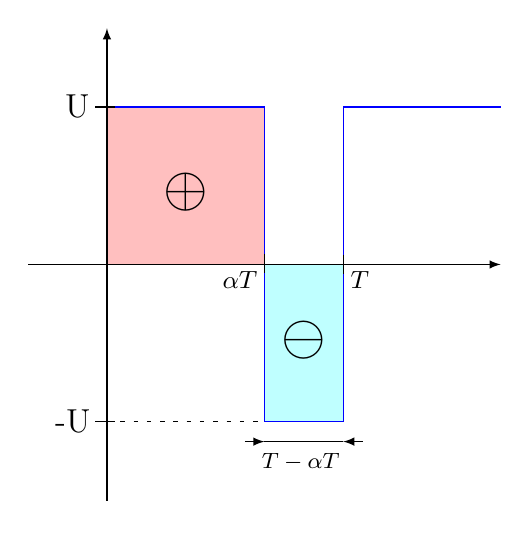
\begin{tikzpicture}
	% Paths, nodes and wires:
	\node[shape=rectangle, fill={rgb,255:red,128;green,255;blue,255}, fill opacity=0.5, minimum width=1cm, minimum height=2cm] at (2.5, -1){};
	\node[shape=rectangle, fill={rgb,255:red,255;green,128;blue,128}, fill opacity=0.5, draw, line width=0.1pt, minimum width=1.996cm, minimum height=1.996cm] at (1, 1){};
	\draw[-latex] (0, -3) -- (0, 3);
	\draw[-latex] (-1, -0) -- (5, 0);
	\path[draw={rgb,255:red,0;green,0;blue,255}] (0, 2) -- (2, 2) -- (2, -2) -- (3, -2) -- (3, 2) -- (5, 2);
	\node[shape=rectangle, minimum width=1.215cm, minimum height=1.09cm] at (1.125, 0.813){} node[anchor=north west, align=left, text width=0.827cm, inner sep=6pt] at (0.5, 1.375){\huge $\oplus$};
	\node[shape=rectangle, minimum width=1.215cm, minimum height=1.09cm] at (2.625, -1.063){} node[anchor=north west, align=left, text width=0.827cm, inner sep=6pt] at (2, -0.5){\huge $\ominus$};
	\draw (2, 0.136) -- (2, -0.114);
	\draw (3.002, 0.126) -- (3.002, -0.124);
	\draw[dash pattern={on 1.6pt off 3.2pt}] (0, -2) -- (2, -2);
	\node[shape=rectangle, minimum width=1.215cm, minimum height=1.09cm] at (-0.25, -2.187){} node[anchor=north west, align=left, text width=0.827cm, inner sep=6pt] at (-0.875, -1.625){\large -U};
	\node[shape=rectangle, minimum width=1.215cm, minimum height=1.09cm] at (-0.125, 1.813){} node[anchor=north west, align=left, text width=0.827cm, inner sep=6pt] at (-0.75, 2.375){\large U};
	\draw (0.097, 2) -- (-0.153, 2);
	\draw (0.102, -2) -- (-0.148, -2);
	\node[shape=rectangle, minimum width=1.215cm, minimum height=1.09cm] at (1.875, -0.437){} node[anchor=north west, align=left, text width=0.827cm, inner sep=6pt] at (1.25, 0.125){\small $\alpha T$};
	\node[shape=rectangle, minimum width=1.215cm, minimum height=1.09cm] at (3.5, -0.437){} node[anchor=north west, align=left, text width=0.827cm, inner sep=6pt] at (2.875, 0.125){\small $ T$};
	\draw[-latex] (1.75, -2.25) -- (2, -2.25);
	\draw[-latex] (3.25, -2.25) -- (3, -2.25);
	\draw (2, -2.25) -- (3, -2.25);
	\node[shape=rectangle, minimum width=1.465cm, minimum height=1.09cm] at (2.5, -2.75){} node[anchor=north west, align=left, text width=1.077cm, inner sep=6pt] at (1.75, -2.187){\footnotesize $T-\alpha T$};
\end{tikzpicture}
    \caption{Signal d’entrée de la MCC}
    \label{circuit:}
\end{figure}
Grâce à la méthode des aires, on peut établir la relation entre la tension d'alimentation du hacheur (ici 48 V) et sa tension moyenne de sortie, on a donc :
\begin{center}
    \begin{tcolorbox}[colframe=red,width=\linewidth]
        \begin{equation}
            <U_{AB}>=\frac{aire\oplus-aire\ominus}{T}=\frac{U\alpha T-U(T-\alpha T)}{T}=(2\alpha-1)U=(2\frac{u_{commande}}{U_M}-1)U
            \label{eq:commande_hach}
        \end{equation}
    \end{tcolorbox}
\end{center}
Nous avons ainsi modélisé le signal fourni par le hacheur par le calcul de sa valeur moyenne. Cela sera particulièrement utile pour les simulations sur Simulink qui ne contient pas de modèle de hacheur intégré.
\subsubsection{Implémentation sous PSIM}
A partir de ce qui a été dit précédemment, on implémente la commande de la manière suivante sur PSIM:
\begin{figure}[H]
    \centering
    \includegraphics[width=0.4\linewidth]{Images/Modelisation/PSIM/Commande_PSIM.jpg}
    \caption{Modélisation de la commande sous PSIM \hyperref[sec:arb]{*}}
    \label{fig:commande_psim}
\end{figure}
\subsubsection{Implémentation sous Matlab/Simulink}
De même, à partir de l'\autoref{eq:commande_hach}, on implémente la commande sur Simulink en changeant la constante $U$ précédente par ce qui est montré en \autoref{fig:commande_matlab}:
\begin{figure}[H]
    \centering
    \includegraphics[width=0.8\linewidth]{Images/Modelisation/MATLAB/Commande_Matlab.jpg}
    \caption{Modélisation de la commande sous Matlab \hyperref[sec:arb]{*}}
    \label{fig:commande_matlab}
\end{figure}
\newpage
\subsection{Etude du régime permanent considérant la commande}
Nous pouvons à présent vérifier la conformité de la modélisation de la commande sur Simulink puis sur PSIM. Pour cela, nous prendrons pour l'exemple un rapport cyclique $\alpha = 0,75$ avec $u_{commande}=11,25V$ et $U_M=15V$.
\subsubsection{Sous Matlab/Simulink}
On peut recalculer sur Matlab, les valeurs finales de nos variables d'états en remplacement $U$ par la valeur de $<U_{AB}>$ établie en (\ref{eq:commande_hach}) et grâce aux valeurs de l'exemple évoquées précédemment. On obtient alors :
\\
$$X'_{\infty}=
    \begin{pmatrix}
        2,2882\space A   \\
        1,78142 \space A \\
        1543 \space tr/min
    \end{pmatrix}
$$
\subsubsection{Sous PSIM}


Testons à présent notre modélisation sur PSIM. Pour cela, nous allons reproduire la formule de $<U_{AB}>$ à l'aide de blocs de la manière suivante :
\begin{figure}[H]
    \centering
    \includegraphics[width=0.7\linewidth]{Images/Modelisation/PSIM/blocs_commande.png}
    \caption{Reproduction de la formule $<U_{AB}>$ sous PSIM \hyperref[sec:arb]{*}}
    \label{fig:model_commande_psim}
\end{figure}

On observe ici la création de 2 signaux : le premier (label C) est le signal MLI évoqué plus tôt qui va piloter le hacheur et en second, on créé le signal $<U_{AB}>=(2\displaystyle\frac{u_{commande}}{U_M}-1)U$ à partir de $u_{commande}$, ici une source de tension continue. Nous pouvons ainsi comparer l'évolution de nos variables d'états avec 2 entrées différentes : l'une est le signal directement fourni par le hacheur et l'autre est le signal de sortie modélisé.\\
\newpage
En \autoref{fig:c_induit_psim_comm}, \autoref{fig:vitesse_psim_comm} et \autoref{fig:vitess_ondulation} sont présentées, l'allure du courant d'induit et de la vitesse avec ces deux signaux:

\begin{figure}[H]
    \centering  \includegraphics[width=1\linewidth,height=10cm]{Images/Modelisation/PSIM/courant_IM_comp_hacheur.png}
    \caption{Courant d'induit moteur avec hacheur (vert) et courant d'induit moteur avec modélisation du hacheur (rouge) \hyperref[sec:arb]{*}}
    \label{fig:c_induit_psim_comm}
\end{figure}
\textit{On a en abscisse le temps en seconde et en ordonnée le courant  en ampère.}

\begin{figure}[H]
    \centering
    \includegraphics[width=1\linewidth]{Images//Modelisation//PSIM/Vitessse_Hacheur.png}
    \caption{Vitesse moteur avec hacheur (vert) et vitesse moteur avec modélisation du hacheur (rouge) \hyperref[sec:arb]{*}}
    \label{fig:vitesse_psim_comm}
\end{figure}
\textit{On a en abscisse le temps en seconde et en ordonnée la vitesse en $tr/min$.}

\begin{figure}[H]
    \centering
    \includegraphics[width=1\linewidth]{Images//Modelisation//PSIM/Ondulation_vitesse_hacheur.png}
    \caption{Zoom sur l'ondulation de vitesse \hyperref[sec:arb]{*}}
    \label{fig:vitess_ondulation}
\end{figure}
\textit{On a en abscisse le temps en seconde et en ordonnée la vitesse en $tr/min$.} \\ \\
On constate plusieurs choses:
\begin{itemize}[label=\textbullet]
    \item Tout d'abord avec le signal directement fourni par le hacheur, on constate  une ondulation sur les deux courbes. Celle-ci est dû au signal du hacheur qui n'est pas continu mais carré.
    \item Malgré cette ondulation, on constate que l'évolution des grandeurs est la même que celle avec la modélisation du hacheur, ce qui confirme la bonne conception de notre hacheur sur PSIM. De plus, la courbe avec modélisation du hacheur est pratiquement la même que celle que nous obtenons sur Matlab avec la même modélisation de la commande. Cela conforte encore notre modèle.
    \item Enfin, les valeurs des grandeurs en régime permanent obtenus avec ces courbes sont cohérentes avec celles calculées via Matlab précédemment.
\end{itemize}
On voit que PSIM nous permet donc de simuler plus finement le système en prenant en compte les ondulations réelles du système.

\section{Dimensionnement et simulation des asservissements}
\subsection{Préliminaire à l'asservissement}
Avant de commencer le dimensionnement de nos asservissements, nous devons légèrement modifier notre modèle. En effet, pour réaliser nos asservissements, on va considérer que l'on se situe autour d'un point d'équilibre et que nous allons linéariser le système autour de ce point d'équilibre. Ainsi, nous ne prendrons pas en compte les éléments invariants à une perturbation $\delta$ sur notre système. De ce fait, nous négligerons dans notre asservissement les frottements secs $2C_0$ et prendrons en compte uniquement le gain du hacheur à une perturbation, soit $\displaystyle \frac{2U}{U_M}=6,4$. On ajustera donc ces éléments dans nos modèles PSIM et Matlab. On utilisera aussi un limiteur de tension pour limiter la tension de commande afin qu'elle ne sorte pas de sa plage de fonctionnement normale.
\newpage
\subsection{Asservissement en courant}
\subsubsection{Calcul du correcteur}
Pour simplifier la réalisation de l'asservissement, nous allons regrouper les différentes parties qui constituent notre schéma bloc global et établir la fonction de transfert en boucle ouverte du courant. On a le schéma bloc suivant :

\begin{figure}[H]
    \centering
    \begin{tikzpicture}[transform shape,scale=0.6]
	% Paths, nodes and wires:
	\node[shape=rectangle, draw, line width=1pt, minimum width=2.465cm, minimum height=1.465cm] at (-6.696, 4){} node[anchor=center, align=center, text width=2.077cm, inner sep=6pt] at (-6.696, 4){\LARGE 6,4};
	\node[shape=rectangle, draw, line width=1pt, minimum width=2.465cm, minimum height=1.465cm] at (0.495, 4){} node[anchor=center, align=center, text width=2.077cm, inner sep=6pt] at (0.495, 4){\LARGE $\frac{1}{R+Lp}$};
	\node[shape=rectangle, draw, line width=1pt, minimum width=1.215cm, minimum height=1.465cm] at (4.37, 4){} node[anchor=center, align=center, text width=0.827cm, inner sep=6pt] at (4.37, 4){\LARGE $K_{\phi}$};
	\node[mixer] at (6.995, 4.003){};
	\node[shape=rectangle, draw, line width=1pt, minimum width=2.465cm, minimum height=1.465cm] at (9.975, 4){} node[anchor=center, align=center, text width=2.077cm, inner sep=6pt] at (9.975, 4){\LARGE $\frac{1}{2Jp}$};
	\node[mixer] at (6.995, 1.513){};
	\node[shape=rectangle, draw, line width=1pt, minimum width=1.215cm, minimum height=1.465cm] at (9.975, 1.5){} node[anchor=center, align=center, text width=0.827cm, inner sep=6pt] at (9.975, 1.5){\LARGE $2f$};
	\node[shape=rectangle, draw, line width=1pt, minimum width=2.735cm, minimum height=1.465cm] at (10.11, -1.25){} node[anchor=center, align=center, text width=2.347cm, inner sep=6pt] at (10.11, -1.25){\LARGE $\frac{K_{\phi}^2}{R+R_{ch}+Lp}$};
	\node[mixer] at (-3.015, 4.013){};
	\node[shape=rectangle, draw, line width=1pt, minimum width=1.215cm, minimum height=1.465cm] at (-3.005, 0.263){} node[anchor=center, align=center, text width=0.827cm, inner sep=6pt] at (-3.005, 0.263){\LARGE $K_{\phi}$};
	\draw[-latex] (1.745, 4) |- (3.745, 4);
	\draw[-latex] (4.995, 4.013) |- (6.495, 4.013);
	\draw[-latex] (7.475, 4.013) |- (8.745, 4.013);
	\draw (11.245, 4.013) -- (13.495, 4.013);
	\draw (13.495, 1.513) -| (13.495, 4.013);
	\node[circ] at (13.495, 1.5){};
	\node[circ] at (13.495, 4.013){};
	\node[circ] at (13.495, -1.237){};
	\draw (13.495, -1.237) -- (13.495, -2.987) -- (-3.005, -2.987);
	\draw[-latex] (-3.005, -2.987) -- (-3.005, -0.487);
	\draw[-latex] (-3.005, 1.013) -| (-3.008, 3.523);
	\draw[-latex] (8.755, -1.227) -- (7.005, -1.227) -- (7.005, 1.023);
	\draw[-latex] (9.35, 1.5) -- (7.495, 1.513);
	\draw[-latex] (6.995, 2.013) -- (6.995, 3.513);
	\draw[-latex] (-2.525, 4.013) -- (-0.755, 4);
	\draw[-latex] (-5.505, 4.013) -- (-3.505, 4.013);
	\node[shape=rectangle, minimum width=0.651cm, minimum height=0.608cm] at (6.717, 3.987){} node[anchor=north, align=center, text width=0.263cm, inner sep=6pt] at (6.717, 4.308){\footnotesize +};
	\node[shape=rectangle, minimum width=0.465cm, minimum height=0.215cm] at (-3.005, 3.763){} node[anchor=north, align=center, text width=0.077cm, inner sep=6pt] at (-3.005, 3.888){\footnotesize -};
	\node[shape=rectangle, minimum width=0.465cm, minimum height=0.215cm] at (7.003, 3.763){} node[anchor=north, align=center, text width=0.077cm, inner sep=6pt] at (7.003, 3.888){\footnotesize -};
	\draw (13.495, 1.513) -| (13.495, -1.237);
	\draw[-latex] (13.495, 1.513) -- (10.745, 1.513) -- (10.6, 1.5);
	\draw (13.495, -1.237) -- (11.495, -1.237);
	\draw (-7.946, 3.895) |- (-10.446, 3.907);
	\node[shape=rectangle, minimum width=2.215cm, minimum height=1.215cm] at (12.441, 3.106){} node[anchor=north west, align=left, text width=1.827cm, inner sep=6pt] at (11.316, 3.731){\textcolor{rgb,255:red,255;green,0;blue,0}{\Large A}};
	\node[shape=rectangle, minimum width=2.215cm, minimum height=1.215cm] at (11.941, 0.731){} node[anchor=north west, align=left, text width=1.827cm, inner sep=6pt] at (10.816, 1.356){\textcolor{rgb,255:red,255;green,0;blue,0}{\Large B}};
	\node[shape=rectangle, minimum width=2.215cm, minimum height=1.215cm] at (12.691, -2.019){} node[anchor=north west, align=left, text width=1.827cm, inner sep=6pt] at (11.566, -1.394){\textcolor{rgb,255:red,255;green,0;blue,0}{\Large C}};
	\node[shape=rectangle, minimum width=0.715cm, minimum height=0.715cm] at (13.5, 7.25){} node[anchor=center, align=center, text width=0.327cm, inner sep=6pt] at (13.5, 7.25){\LARGE $\delta(\Omega)$};
	\node[shape=rectangle, minimum width=2.215cm, minimum height=1.215cm] at (14.691, 3.856){} node[anchor=north west, align=left, text width=1.827cm, inner sep=6pt] at (13.566, 4.481){\Large S};
	\node[shape=rectangle, minimum width=0.59cm, minimum height=0.572cm] at (6.15, 4.553){} node[anchor=north west, align=left, text width=0.202cm, inner sep=6pt] at (5.838, 4.857){\LARGE e};
	\node[shape=rectangle, minimum width=2.215cm, minimum height=1.215cm] at (8.566, 4.231){} node[anchor=north west, align=left, text width=1.827cm, inner sep=6pt] at (7.441, 4.856){\LARGE $\varepsilon$};
	\draw[-latex] (13.495, 4.013) -| (13.5, 6.75);
	\draw[-latex] (3, 4) -- (3, 7) -- (5, 7);
	\node[shape=rectangle, minimum width=0.965cm, minimum height=1.215cm] at (5.5, 6.875){} node[anchor=north west, align=left, text width=0.577cm, inner sep=6pt] at (5, 7.5){\LARGE $\delta(i_m)$};
	\node[shape=rectangle, minimum width=0.965cm, minimum height=1.215cm] at (-11, 4.25){} node[anchor=north west, align=left, text width=0.577cm, inner sep=6pt] at (-11.5, 4.875){\LARGE $\delta({u_{commande}})$};
	\node[shape=rectangle, minimum width=0.651cm, minimum height=0.608cm] at (7.25, 1.479){} node[anchor=north, align=center, text width=0.263cm, inner sep=6pt] at (7.25, 1.801){\footnotesize +};
	\node[shape=rectangle, minimum width=0.651cm, minimum height=0.608cm] at (7, 1.234){} node[anchor=north, align=center, text width=0.263cm, inner sep=6pt] at (7, 1.555){\footnotesize +};
	\node[shape=rectangle, minimum width=0.651cm, minimum height=0.608cm] at (-3.29, 3.985){} node[anchor=north, align=center, text width=0.263cm, inner sep=6pt] at (-3.29, 4.307){\footnotesize +};
	\node[shape=rectangle, minimum width=2.215cm, minimum height=1.215cm] at (2.875, 3.25){} node[anchor=north west, align=left, text width=1.827cm, inner sep=6pt] at (1.75, 3.875){\textcolor{rgb,255:red,255;green,0;blue,0}{\Large D}};
\end{tikzpicture}
    \caption{Schéma-bloc du système global}
\end{figure}

A partir de cette structure, nous pouvons établir la fonction de transfert souhaitée. Nous allons dans un premier temps établir une fonction de transfert $H$ qui sera le rapport entre la vitesse $\Omega$ et le courant $i_m$. Nous pouvons écrire les équations suivantes :

\begin{equation}
    \begin{cases}
        $$\varepsilon=e-B \cdot S-C\cdot S$$ \\
        $$S=A\cdot \varepsilon=A(e-(B+C)S) $$
    \end{cases}
    \label{eq:re}
\end{equation}

On en tire l'expression suivante :
$$S=\frac{A\cdot e}{1+A(B+C)}$$

En nommant $H=K_{\phi} \cdot\displaystyle \frac{A}{1+A(B+C)}$, on a finalement :

$$H=\frac{\Omega(p)}{i_m(p)}=K_{\phi} \cdot\displaystyle \frac{A}{1+A(B+C)}$$

\vspace{10px}

Nous pouvons alors simplifier le schéma bloc de la manière suivante :

\begin{figure}[H]
    \centering
    \begin{tikzpicture}[transform shape,scale=0.75]
	% Paths, nodes and wires:
	\node[shape=rectangle, draw, line width=1pt, minimum width=2.465cm, minimum height=1.465cm] at (-6.226, 3.484){} node[anchor=center, align=center, text width=2.077cm, inner sep=6pt] at (-6.226, 3.484){\LARGE 6,4};
	\node[shape=rectangle, draw, line width=1pt, minimum width=2.465cm, minimum height=1.465cm] at (1, 3.5){} node[anchor=center, align=center, text width=2.077cm, inner sep=6pt] at (1, 3.5){\LARGE $\frac{1}{R+Lp}$};
	\node[shape=rectangle, draw, line width=1pt, minimum width=2.465cm, minimum height=1.465cm] at (6.202, 3.468){} node[anchor=center, align=center, text width=2.077cm, inner sep=6pt] at (6.202, 3.468){\LARGE H};
	\node[mixer] at (-2.5, 3.49){};
	\node[shape=rectangle, draw, line width=1pt, minimum width=1.215cm, minimum height=1.465cm] at (-2.5, 1.25){} node[anchor=center, align=center, text width=0.827cm, inner sep=6pt] at (-2.5, 1.25){\LARGE $K_{\phi}$};
	\draw (7.452, 3.468) -| (10.006, 3.5);
	\draw (10.006, 1) -| (10.006, 3.5);
	\node[circ] at (10.006, 3.468){};
	\draw[-latex] (-4.976, 3.484) -- (-2.976, 3.484);
	\node[shape=rectangle, minimum width=0.465cm, minimum height=0.215cm] at (-2.497, 3.22){} node[anchor=north, align=center, text width=0.077cm, inner sep=6pt] at (-2.497, 3.345){\footnotesize -};
	\draw (-7.476, 3.471) |- (-9.976, 3.484);
	\node[shape=rectangle, minimum width=0.715cm, minimum height=0.715cm] at (10.01, 6.612){} node[anchor=center, align=center, text width=0.327cm, inner sep=6pt] at (10.01, 6.612){\LARGE $\delta(\Omega)$};
	\node[shape=rectangle, minimum width=2.215cm, minimum height=1.215cm] at (11.25, 3.375){} node[anchor=north west, align=left, text width=1.827cm, inner sep=6pt] at (10.125, 4){\Large S};
	\draw[-latex] (10.006, 3.468) -| (10.01, 6.237);
	\draw[-latex] (3.5, 3.5) -| (3.481, 6.439) -- (5.481, 6.439);
	\node[shape=rectangle, minimum width=0.965cm, minimum height=1.215cm] at (5.981, 6.314){} node[anchor=north west, align=left, text width=0.577cm, inner sep=6pt] at (5.481, 6.939){\LARGE $\delta(i_m)$};
	\node[shape=rectangle, minimum width=0.965cm, minimum height=1.215cm] at (-10.519, 3.689){} node[anchor=north west, align=left, text width=0.577cm, inner sep=6pt] at (-11.019, 4.314){\LARGE $\delta(u_{commande})$};
	\node[shape=rectangle, minimum width=0.651cm, minimum height=0.608cm] at (-2.795, 3.464){} node[anchor=north, align=center, text width=0.263cm, inner sep=6pt] at (-2.795, 3.786){\footnotesize +};
	\draw[-latex] (-2.514, 2.006) -| (-2.5, 3);
	\draw[-latex] (10, 1) -- (10, -0.5) -- (-2.5, -0.5) -- (-2.5, 0.5);
	\draw[-latex] (2.25, 3.5) -- (5, 3.5);
	\draw[-latex] (-2.01, 3.49) -- (-0.25, 3.5);
	\node[circ] at (3.481, 3.5){};
\end{tikzpicture}
    \caption{Schéma-bloc simplifié du système global}
\end{figure}
\newpage
Nous pouvons finalement établir l'expression du courant d'induit moteur en fonction de la tension de commande :

\begin{center}
    \begin{tcolorbox}[
            colframe=red,
            width=\linewidth/2,
        ]
        \begin{equation}
            \delta(i_m)=6,4\cdot \frac{\displaystyle\frac{1}{R+Lp}}{1+\displaystyle\frac{K_{\phi}^2\cdot H}{R+Lp}}\cdot \delta(u_{commande})
            \label{eq:FT_courant}
        \end{equation}
    \end{tcolorbox}
\end{center}

A présent, il convient de comparer l'exactitude de notre modélisation du courant sur Simulink. Nous avons le schéma-bloc suivant sur Simulink :

\begin{figure}[H]
    \centering
    \includegraphics[width=1\linewidth]{Images//Modelisation//MATLAB/comparaison_courant_simulink.png}
    \caption{Schéma-bloc Simulink \hyperref[sec:arb]{*}}
    \label{fig:exactitude}
\end{figure}

La partie basse correspond au schéma-bloc complet du système et au-dessus, le bloc $I$ correspond à la fonction de transfert établie plus haut sur l'\autoref{eq:FT_courant}. Le facteur $0,99$ permettra de mieux visualiser les deux courbes sur le \textit{scope}. On réalise un essai indiciel:
\begin{figure}[H]
    \centering
    \includegraphics[width=0.8\linewidth]{Images//Modelisation//MATLAB/Comparaison_scope_courant.png}
    \caption{Comparaison du courant d'induit issu du schéma global et du modèle \hyperref[sec:arb]{*}}
    \label{fig:comp_courant_ass_c}
\end{figure}

On observe une correspondance exacte entre les deux courbes ce qui témoigne de la bonne modélisation du courant d'induit à partir de la fonction de transfert en boucle ouverte.

\vspace{10px}

Le modèle maintenant établi et validé, nous pouvons procéder à son asservissement. Nous avons le schéma bloc suivant :

\begin{figure}[H]
    \centering
    \includegraphics[width=0.8\linewidth]{Images//Modelisation//MATLAB/schema_asser_courant.png}
    \caption{Boucle fermée de courant \hyperref[sec:arb]{*}}
    \label{fig:sch_bloc_PID_I_matlab}
\end{figure}

Grâce à la modélisation effectuée précédemment, ce schéma est très simplifié : le correcteur va nous permettre d'ajuster la réponse du courant selon notre cahier des charges. Notre fonction de transfert est en pratique trop complexe pour être étudiée à la main, nous allons donc utiliser l'outil \textit{PID Tuner} de Simulink qui va calculer automatiquement un correcteur selon nos préférences. On rappelle que l'on souhaite un temps de réponse à 5 $\%$ égal à au moins 10 fois la période du signal MLI qui pilote le hacheur. La fréquence de ce signal est fixée à $f_{MLI}=20 \space kHz$ d'où $T_{MLI}= \frac{1}{f_{MLI}}=5\times10^{-5} \space s$. Nous devons donc fixer $t_{r5\%}=10\times T_{MLI}=5\times 10^{-4} s$. On rappelle que l'on devra limiter le dépassement entre 10 $\%$ et 20 $\%$ de la valeur finale.

\vspace{10px}

Ainsi grâce au \textit{PID Tuner}, on règle la réponse en boucle fermée pour qu'elle soit robuste, c'est-à-dire peu sensible aux perturbations et assez rapide pour correspondre à notre cahier des charges. Nous obtenons les valeurs suivantes :
$$PI(p)=P+I\frac{1}{p}$$
$$P=6,2186$$
$$I=41446~s^{-1}$$

La réponse à un essai indiciel est la suivante :

\begin{figure}[H]
    \centering
    \includegraphics[width=1\linewidth]{Images//Modelisation//MATLAB/asserv_courant.png}
    \caption{Réponse asservie du courant d'induit \hyperref[sec:arb]{*}}
    \label{fig:rep_asservie_i_matlab}
\end{figure}

La réponse correspond bien à nos attentes avec un dépassement maximum de 14,8 $\%$ et un temps de réponse effectif de 383 $\mu s$, inférieur au temps de réponse maximum imposé de 500 $\mu s$.

\subsubsection{Vérification du correcteur}
Nous allons maintenant vérifier sur PSIM que notre correcteur a bien été dimensionné.
On réalise donc l'asservissement sur PSIM avec les mêmes valeurs de correcteur que trouvées précédemment à l'aide du schéma suivant:
\begin{figure}[H]
    \centering
    \includegraphics[width=1\linewidth]{Images//Modelisation//PSIM/Correcteur_PSIM_Ass.png}
    \caption{Schéma de vérification de l'asservissement de courant sur PSIM \hyperref[sec:arb]{*}}
    \label{fig:schem_verif_i_asser_psim}
\end{figure}
Nous avons la partie du bas qui simule le correcteur avec le hacheur modélisé et la partie juste au dessus qui utilise le hacheur directement. L'objectif est de voir ici si la réponse à une perturbation avec le hacheur  et le correcteur suit la même évolution que la modélisation avec le même correcteur.
\begin{figure}[H]
    \centering
    \includegraphics[width=1\linewidth]{Images/Modelisation/PSIM/reponse_psim_ass_i.png}
    \caption{Courbes de vérification de l'asservissement de courant sur PSIM \hyperref[sec:arb]{*}}
    \label{fig:rep_psim_ass_i}
\end{figure}
En vert, on a la courbe avec le hacheur modélisé et en rouge, la courbe avec le hacheur. Comme nous avons considéré être autour d'un  point d'équilibre, il est impossible de comparer les réponses à la mise en route du système, il faut donc comparer les réponse à une perturbation en régime établi comme sur la \autoref{fig:rep_psim_ass_i}. On constate que les réponses suivent la même évolution, ce qui valide le calcul de notre correcteur.
\\ \\
\textit{On a bien pris soin de s'assurer que l'asservissement avec la modélisation du hacheur sur PSIM était équivalente à celle sur Matlab (temps de réponse, gain statique, dépassement) avant d'effectuer les comparaisons précédentes.}


\subsection{Asservissement de vitesse}
Pour l'asservissement de vitesse, étant donné que nous utiliserons deux types de capteur qui seront susceptibles de ne pas avoir les mêmes gains, nous expliciterons dans un premier temps la démarche et la réflexion en faisant l'hypothèse que nous avons un gain de capteur unitaire. Par la suite, il nous suffira simplement de prendre en compte les gains \textit{(ou le gain si les capteurs possèdent le même gain)} des capteurs et d'effectuer la même démarche. Ainsi, lors de la prise en compte des capteurs, nous expliciterons uniquement la validité des résultats et non plus la démarche qui sera donc la même que celle présentée en amont.
\subsubsection{Démarche globale}
\paragraph{Calcul du correcteur} \mbox{}\\ \\
De manière similaire à l’asservissement de courant, nous pouvons déterminer la fonction de transfert en boucle fermée équivalente globale pour la vitesse. Celle-ci se calcule grâce à la formule de Black, non plus au niveau de la sortie de courant mais bien celle de vitesse.
\\
\\
Si nous reprenons les écritures précédentes, elle peut s’écrire :

\[\frac{K_\phi\cdot H\cdot D}{1+K_\phi\cdot H\cdot D}\]

A l'aide de Matlab, nous pouvons rapidement calculer cette fonction. Il s'agit d'une fonction de transfert du huitième ordre. Lorsque nous simulons notre système en remplaçant notre schéma bloc par cette seule fonction, voici ce que nous obtenons.

\begin{figure}[H]
    \centering
    \includegraphics[width=1\linewidth]{Images//Modelisation//MATLAB/Asservissemrnt vitesse 8e ordre comparaison.png}
    \caption{Fonction du huitième ordre \hyperref[sec:arb]{*}}
    \label{fig:fun_ordre_hut}
\end{figure}

Nous avons rajouté un facteur 0,99 à la fonction de transfert nouvellement calculée afin de pouvoir discerner nos deux courbes. On remarque effectivement que cette fonction est la bonne modélisation de notre système.
\\
\\
Seulement, cette fonction a été calculée à partir de H, une fonction de transfert du troisième ordre : cela peut rendre sa manipulation fastidieuse, particulièrement lors du calcul du correcteur. Pour résoudre ce problème, nous pouvons réaliser une simplification d'ordre physique.
La constante de temps de l'inductance de la la génératrice étant très rapide, nous pouvons simplement la négliger devant le système complet. Nous pouvons donc simplifier les expressions de certaines fonctions en supposant L nulle.
\\
On peut donc dans la modélisation de la génératrice modifié la fonction que nous avions appelée "$C$", celle-ci devient:
\[C = \frac{K_{\phi}^2}{R+R_{ch}+\bcancel{Lp}} = \frac{K_{\phi}^2}{R+R_{ch}}\]
On remarque que C est à présent une constante, nous pouvons alors l'additionner à notre autre constante $B = 2f$.Nous obtenons ainsi une nouvelle constante que nous noterons \(f_{eq} =\displaystyle \frac{K_{\phi}^2}{R+R_{ch}} +2f \).
\\
\\
Ensuite, nous pouvons calculer la nouvelle fonction de transfert du point de vue de la vitesse. Celle-ci se calcule aisément par la formule de Black suivante :
\[G = \frac{A}{1+A \cdot f_{eq}} = \frac{\frac{1}{2Jp}}{1+\frac{1}{2Jp}f_{eq}} = \frac{1}{2Jp+f_{eq}}\]
\\
\\
On se retrouve maintenant avec une fonction de transfert du premier ordre, bien plus simple à manipuler que H. Néanmoins,  cette approximation pourrait être trop "simplificatrice", comparons donc nos 3 courbes jusqu'ici obtenues afin de valider notre modèle.
\\
\\
Pour ce faire, calculons la nouvelle fonction de transfert en boucle fermée. En effet, $G$ est la nouvelle expression de la fonction que nous avions appelée H. On reprend alors l'expression que nous avions en remplaçant H par $G$ :

\[\frac{K_\phi\cdot G\cdot D}{1+K_\phi\cdot G\cdot D}\]

Nous obtenons une fonction de transfert en boucle fermée du quatrième ordre.
\\
Comparons maintenant nos 3 courbes, celle sans avoir simplifié le schéma bloc, celle en ayant simplifié mais en ayant gardé L non nul, et celle avec le  $L$ de la génératrice nul.
Notons qu'un facteur 0.99 et 1.01 ont été ajoutés aux courbes simplifiées pour une meilleure visibilité.
\\
On obtient :
\begin{figure}[H]
    \centering
    \includegraphics[width=1\linewidth]{Images//Modelisation//MATLAB/Comparaison 3 courbes vitesse matlab.png}
    \caption{Comparaison des 3 modèles \hyperref[sec:arb]{*}}
    \label{fig:com_3_mod}
\end{figure}
Au vue de ces courbes, il va sans dire que notre modèle avec une fonction du premier ordre plutôt que du troisième ordre est parfaitement justifié.
\\
\\
Avant de calculer l'asservissement, il est possible d'effectuer une dernière simplification dans le schéma bloc qui va alléger nos calculs.
Nous savons que l'asservissement de vitesse ne peut se faire sans celui du courant, il faudrait alors prendre toute la partie précédente en compte ici pour calculer notre correcteur et nos fonctions de transfert équivalentes. \\
Cependant, rappelons nous que le temps de réponse de la boucle de courant est de l'ordre de la centaine de µs tandis que celui la vitesse est de l'ordre du dixième de seconde. Ainsi, comme $\tau_{courant}<<\tau_{vitesse}$, nous pouvons assimiler l'entièreté de la boucle de courant à un gain unitaire, cette dernière n'ayant quasiment aucun impact sur le réponse en vitesse de notre système. \\
Maintenant que ce modèle a été validé, nous pouvons passer à l'asservissement. L'avantage que nous avons à présent, est que nous pouvons calculer facilement à la main les coefficients de notre correcteur proportionnel-intégral. On a donc le schéma bloc suivant:
\begin{figure}[H]
    \centering
    \begin{tikzpicture}[
    block/.style = {draw, rectangle, minimum height=1cm, minimum width=1.8cm, align=center},
    sum/.style   = {draw, circle, node distance=1cm, inner sep=0pt, minimum size=6mm},
    >={Stealth}
]

% Noeuds
\node[sum] (sum) {};
\node[block, right=1.5cm of sum] (C) {$C_\Omega(p)$};
\node[block, right=1.8cm of C] (K) {$K_\Phi$};
\node[block, right=1.8cm of K] (G) {$\dfrac{1}{2Jp + f_{eq}}$};
\node[right=1.2cm of G] (output) {$\Omega$};

% Signes du sommateur
\node at ([xshift=-0.1cm,yshift=0.1cm]sum.center) {\small $+$};
\node at ([xshift=-0cm,yshift=-0.15cm]sum.center) {\small $-$};

% Connexions principales
\draw[->] (sum) -- node[above] {} (C);
\draw[->] (C) -- node[above] {$I_{ref} = i_M$} (K);
\draw[->] (K) -- (G);
\draw[->] (G) -- (output);

% Boucle de rétroaction
\draw[->] (output) |- ++(0,-1.4) -| (sum);

% Entrée
\draw[->] ++(-1.2,0) node[left] {$\Omega_{ref}$} -- (sum);

\end{tikzpicture}
    \caption{Schéma-bloc de l'asservissement de vitesse final}
\end{figure}

Rappelons les calculs :
\[
    F(p) = \frac{C(p)G(p)}{1 + C(p)G(p)}
    = \frac{ K_i \dfrac{1+\tau p}{\tau p} \dfrac{A}{1+\tau p}  }{ 1 + K_i \dfrac{1+\tau p}{\tau p} \dfrac{A}{1+\tau p} }
    = \frac{ \dfrac{K_i A}{\tau p} }{ 1 + \dfrac{K_i A}{\tau p} }
    = \frac{1}{1 + \dfrac{\tau}{K_i A} p}
    = \frac{K_{BF}}{1 + \tau_{BF} p}
\]
Où C(p) est le correcteur, T(p) est la fonction de transfert de notre système en boucle ouverte et H(p) est la fonction de transfert de notre système asservi en boucle fermée.
\\
\\
On peut réécrire l'expression de $G$ :


\[\frac{1}{2Jp+f_{eq}} = \frac{\frac{1}{f_{eq}}}{1+\frac{2J}{f_{eq}}p}\]

On en déduit

$$\tau_{BO} = \frac{2J}{f_{eq}}$$
\\
De même on trouve $A=\dfrac{K_{Phi}}{f_{eq}}$. Il ne faut pas oublier le facteur $K_{Phi}$ dans la formule de Black.

De ça, on calcule ensuite $\tau_{BF} = \dfrac{\tau_{BO}}{K_iA} =\frac{\frac{2J}{f_{eq}}}{K_i\cdot\frac{1}{f_{eq}}\cdot K_{Phi}}$

Or, le cahier des charges stipule un temps de réponse en boucle fermée 3 fois inférieur à celui en boucle ouverte, on en déduit alors que $K_i\cdot\frac{1}{f_{eq}}\cdot K_{Phi} = 3 \rightarrow K_i = \frac{3f_{eq}}{K_{Phi}} = 0,0354$.
\\
\\
Précisons que lors des calculs, nous avons volontairement choisi $T_i=\tau_{BO}$ afin de simplifier l'expression.
Nous savons que cette méthode n'est pas la plus optimale, mais elle fournit un résultat satisfaisant pour ce que nous cherchons. Nous comparerons nos calculs aux résultats trouvés avec le PID Tuner pour s'en assurer.
\newpage
Nos coefficients de correcteur maintenant calculés, testons notre asservissement sur Matlab.
\\
Pour ce faire, de façon analogue à l'asservissement de courant, nous venons créer une simple boucle de rétroaction munie d'un correcteur PI en essai indiciel.
\begin{figure}[H]
    \centering
    \includegraphics[width=1\linewidth]{Images//Modelisation//MATLAB/Asservissement vitesse PI Matlab.png}
    \caption{Asservissement simplifié de la vitesse}
    \label{fig:placeholder}
\end{figure}

Ici, dans le PI, nous remplissons $P =K_i = 0,0354$ et  $ I = \dfrac{1}{\tau_{BO}} = 27,1~s^{-1}$.
\\
\\
Lorsque nous lançons la simulation avec un échelon de 1, nous obtenons la courbe suivante :

\begin{figure}[H]
    \centering
    \includegraphics[width=1\linewidth]{Images//Modelisation//MATLAB/Vitesse_Asservie Graph Matlab PI calculé.png}
    \caption{Graphe de la vitesse asservie \hyperref[sec:arb]{*}}
    \label{fig:vi_ass}
\end{figure}

A l'aide des curseurs, nous pouvons déterminer le temps de réponse à 5\%, ici nous le mesurons à 0.1085s.
Rappelons $tr_{5\%BF} = 3\tau_{BF} = 3\times \displaystyle \frac{\frac{2J}{f_{eq}}}{K_i\times\frac{1}{f_{eq}}\times K_{Phi}} = \frac{2J}{f_{eq}}= 0.1107s$

On trouve ce que l'on cherchait, le correcteur PI est donc bien dimensionné.
\\
\\
Avec le PID Tuner, nous trouvons :
\\
$$K_i = 0,0110$$

$$T_i = 0,0142s$$
\paragraph{Vérification du correcteur} \mbox{}\\ \\
Comme précédemment pour le courant, nous allons vérifier notre asservissement sur PSIM. Étant donné que pour calculer notre correcteur de vitesse, nous avons fait l'hypothèse que le courant s'établissait instantanément, il ne faut donc pas oublier de tester l'asservissement de vitesse \textbf{avec} l'asservissement de courant. Nous aurons donc ici notre système complet asservi. Voici le schéma de ce dernier sur la figure suivante:
\begin{figure}[H]
    \centering
    \includegraphics[width=1\linewidth]{Images//Modelisation//PSIM/corr_vitesse_glob_psim.png}
    \caption{Vérification de l'asservissement de vitesse: Schéma PSIM \hyperref[sec:arb]{*} }
    \label{fig:sch_vit_psim_ass_cor_veri}
\end{figure}
Nous avons la partie du bas qui simule le correcteur avec le hacheur modélisé et la partie juste au dessus qui utilise le hacheur directement. Le premier correcteur à gauche est celui de vitesse et le deuxième à droite, celui de courant. Comme précédemment, l'objectif est de voir ici si la réponse à une perturbation avec le hacheur  et le correcteur suit la même évolution que la modélisation avec le même correcteur.
\begin{figure}[H]
    \centering
    \includegraphics[width=1\linewidth]{Images//Modelisation//PSIM/courbe_vitesse_corrige_psim.png}
    \caption{Courbes de vérification de l’asservissement de vitesse sur PSIM \hyperref[sec:arb]{*}}
    \label{fig:comp_courbe_v_asser}
\end{figure}
En vert, on a la courbe avec le hacheur modélisé et en rouge, la courbe avec le hacheur. Comme nous avons considéré être autour d’un point d’équilibre, il est impossible de comparer les réponses à la mise en route du système, il faut donc comparer les réponse à une perturbation en régime établi comme sur la \autoref{fig:comp_courbe_v_asser}. On constate que les réponses suivent la même évolution, ce qui valide le calcul de notre correcteur. \\ \\
\textit{On a bien pris soin de s’assurer que l’asservissement avec la modélisation du hacheur sur PSIM était équi-
    valente à celle sur Matlab (temps de réponse, gain statique, dépassement) avant d’effectuer les comparaisons précédentes.}


